%%%%%%%%%%%%%%%%%%%%%%%%%%%%%%%%%%%%%%%%%%%%%%%%%%%%%%%%%%%%%%%%%%%%%%%%%%%%%%%%%%
\begin{frame}[fragile]\frametitle{}
\begin{center}
{\Large Cypher}
\end{center}
\end{frame}


%%%%%%%%%%%%%%%%%%%%%%%%%%%%%%%%%%%%%%%%%%%%%%%%%%%%%%%%%%%
\begin{frame}[fragile]\frametitle{Introduction}
A pattern matching query language made for graphs

\begin{itemize}
\item Declarative: say, what you want? and not how to search for the answer (Imperative)
\begin{itemize}
\item  Allowing you to focus on your domain instead of getting lost in the syntax of database access.
\item An expressive and efficient queries to handle needed create, read, update, and delete functionality (also know as CRUD operations
\end{itemize}
\item Expressive
\item Pattern-Matching : ASCI Art
\end{itemize}

\end{frame}

%%%%%%%%%%%%%%%%%%%%%%%%%%%%%%%%%%%%%%%%%%%%%%%%%%%%%%%%%%%
\begin{frame}[fragile]\frametitle{Use Case}

Movie Dataset

\begin{itemize}
\item The graph contains nodes with the labels Person and Movie. 
\item Person nodes have several types of relationships to Movie nodes. 
\item A Person node can have a FOLLOWS relationship to another Person node.
\end{itemize}


\begin{center}
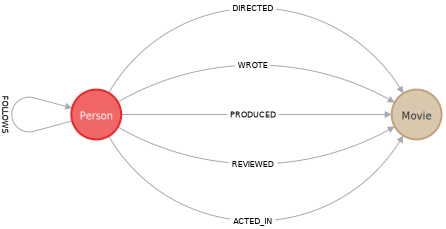
\includegraphics[width=0.8\linewidth,keepaspectratio]{neo4j62}
\end{center}	  


{\tiny (Ref: Introduction to cypher fundamentals  - neo4j)}

\end{frame}

%%%%%%%%%%%%%%%%%%%%%%%%%%%%%%%%%%%%%%%%%%%%%%%%%%%%%%%%%%%
\begin{frame}[fragile]\frametitle{Representation}


\begin{itemize}
\item Nodes are represented in round brackets \lstinline|() or (node variable name)|, similar to a circle on witheboard. An anonymous node \lstinline|()| represents one or more nodes during a query processing where there are no restrictions of the type of the node
\item Labels are used as type to group nodes and filter queries against the graph and is defined with a colon \lstinline|(:Label)|. A node can have zero or more labels for example \lstinline|(node), (node:Label), (node:Label1:Label2), (:Label), (:Label1:Label2)|.
\item Relationships are represented as arrow with its label in square bracket in between \lstinline|-[:RELATIONSHIP]->|
\item Aliases or variable names are  used to referred elements to later in the query defined by a name before a name like \lstinline|(node1:Label1)<-[relationship:RELATIONSHIP]-(node2:Label2)| where \lstinline|node1, node2| and \lstinline|relationship| are aliases.
\item he properties of a node are accessed using \lstinline|{variable}.{property_key}|, for example \lstinline|emil.name or movie.title|.
\end{itemize}

{\tiny (Ref: Learning Neo4j - Wabri Github)}


\end{frame}

%%%%%%%%%%%%%%%%%%%%%%%%%%%%%%%%%%%%%%%%%%%%%%%%%%%%%%%%%%%
\begin{frame}[fragile]\frametitle{Representation}


\begin{center}
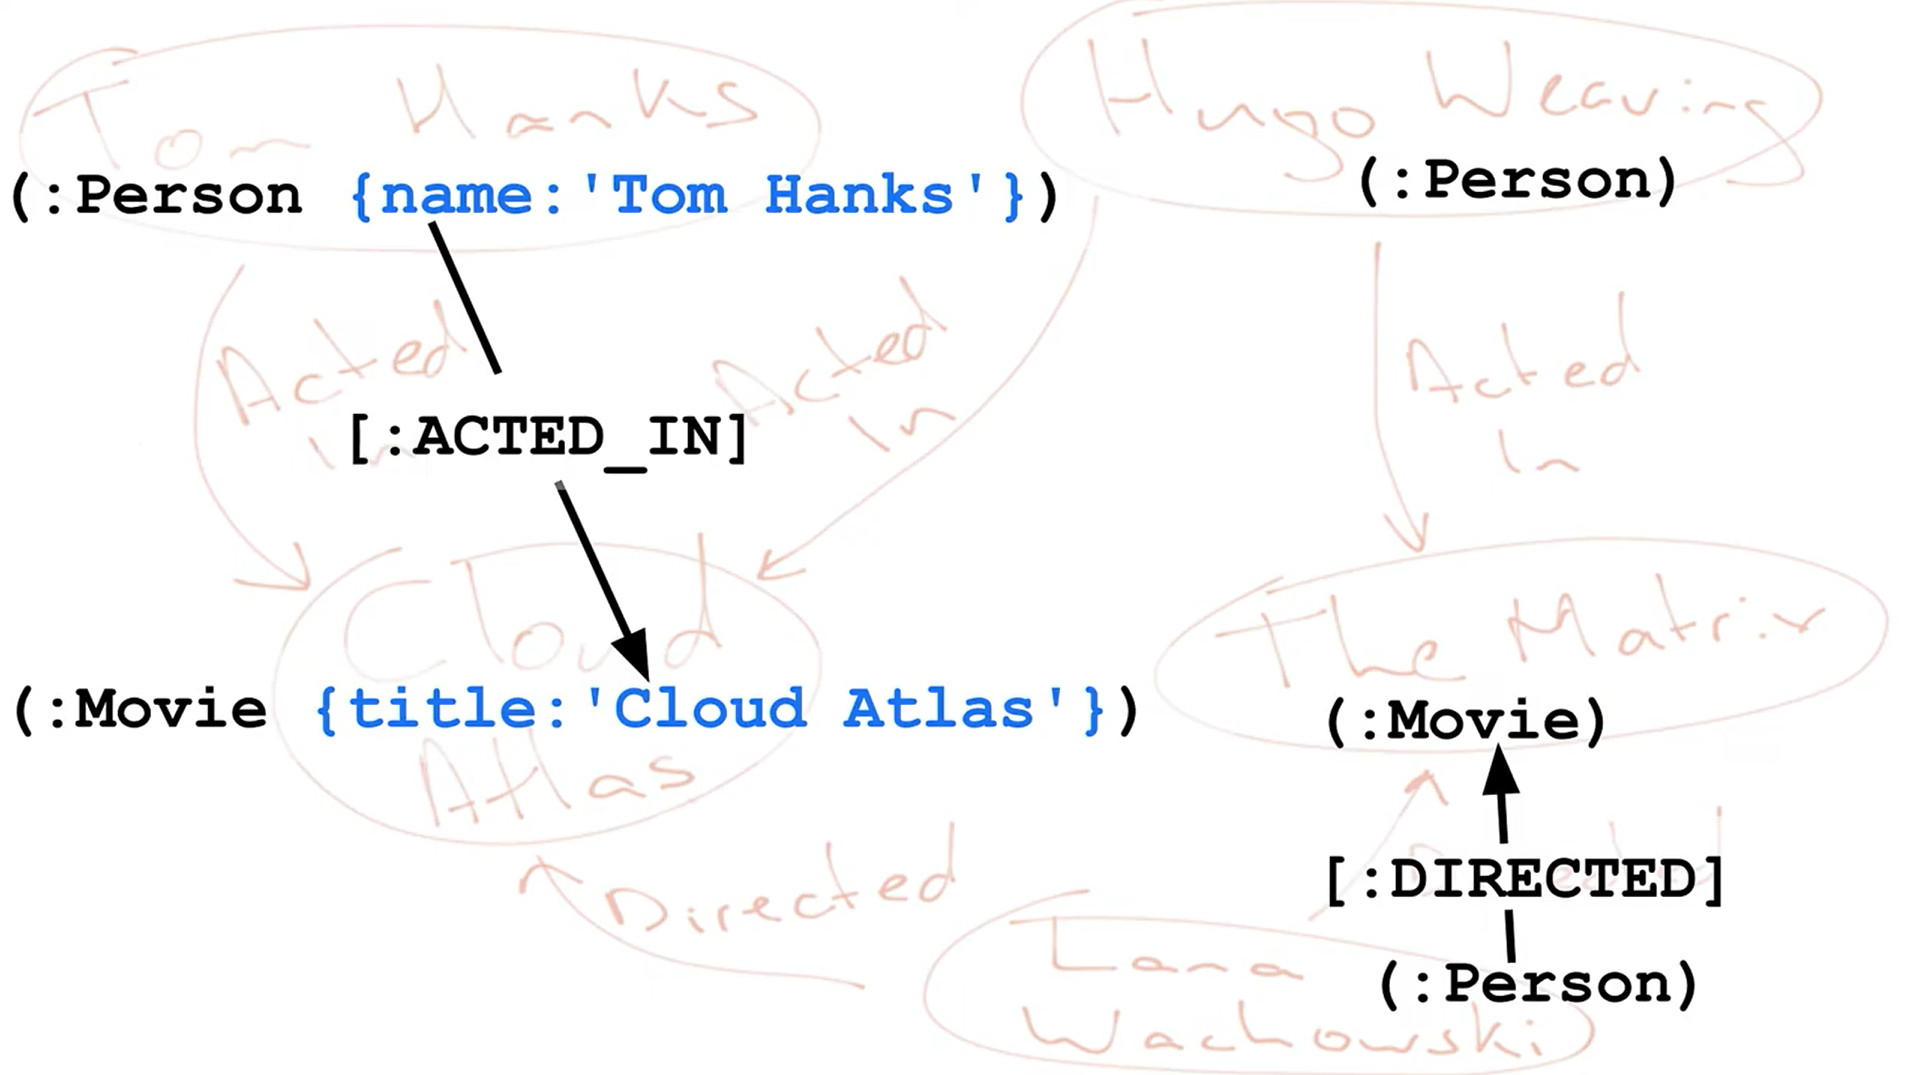
\includegraphics[width=\linewidth,keepaspectratio]{neo4j63}
\end{center}	  


{\tiny (Ref: Introduction to cypher fundamentals  - neo4j)}

\end{frame}


%%%%%%%%%%%%%%%%%%%%%%%%%%%%%%%%%%%%%%%%%%%%%%%%%%%%%%%%%%%%%%%%%%%%%%%%%%%%%%%%%%
\begin{frame}[fragile]\frametitle{}
\begin{center}
{\Large Reading}
\end{center}
\end{frame}


%%%%%%%%%%%%%%%%%%%%%%%%%%%%%%%%%%%%%%%%%%%%%%%%%%%%%%%%%%%
\begin{frame}[fragile]\frametitle{Basic Syntax}

\begin{center}
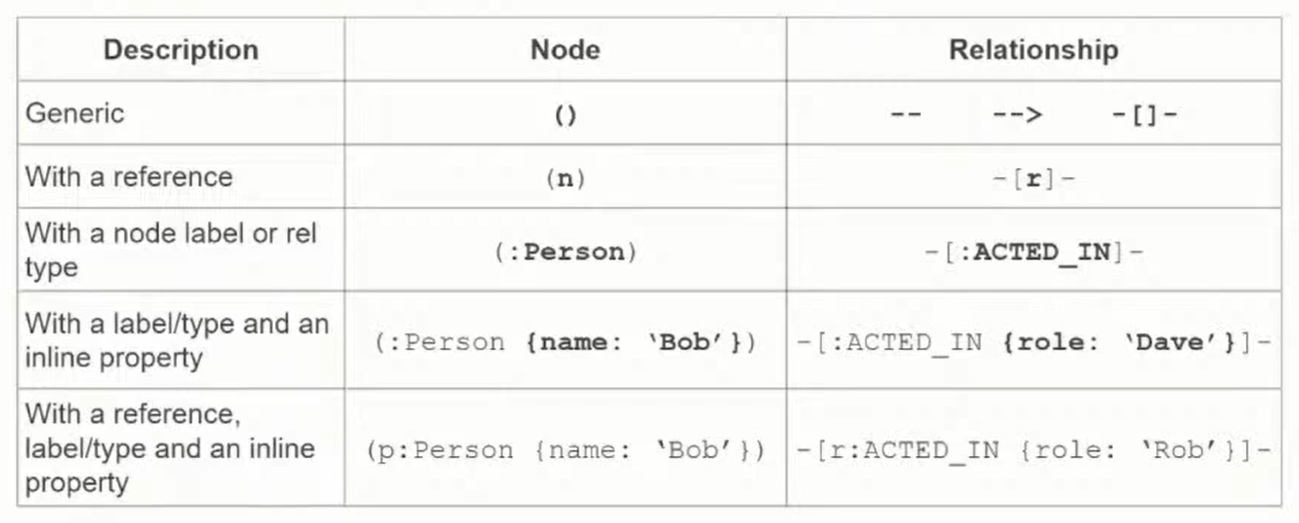
\includegraphics[width=\linewidth,keepaspectratio]{neo4j9}
\end{center}	  


{\tiny (Ref: Introduction to Neo4j - a hands-on crash course  - neo4j)}

\end{frame}

%%%%%%%%%%%%%%%%%%%%%%%%%%%%%%%%%%%%%%%%%%%%%%%%%%%%%%%%%%%
\begin{frame}[fragile]\frametitle{Retrieval}


\begin{itemize}
\item Pattern specification for MATCH command, to retrieve data in graph.
\item Find and return person $p$ and movie $m$
\item First finds $p$ with given name, then goes to all relationships with given type and then finds $m$ which matches given title.
\end{itemize}


\begin{center}
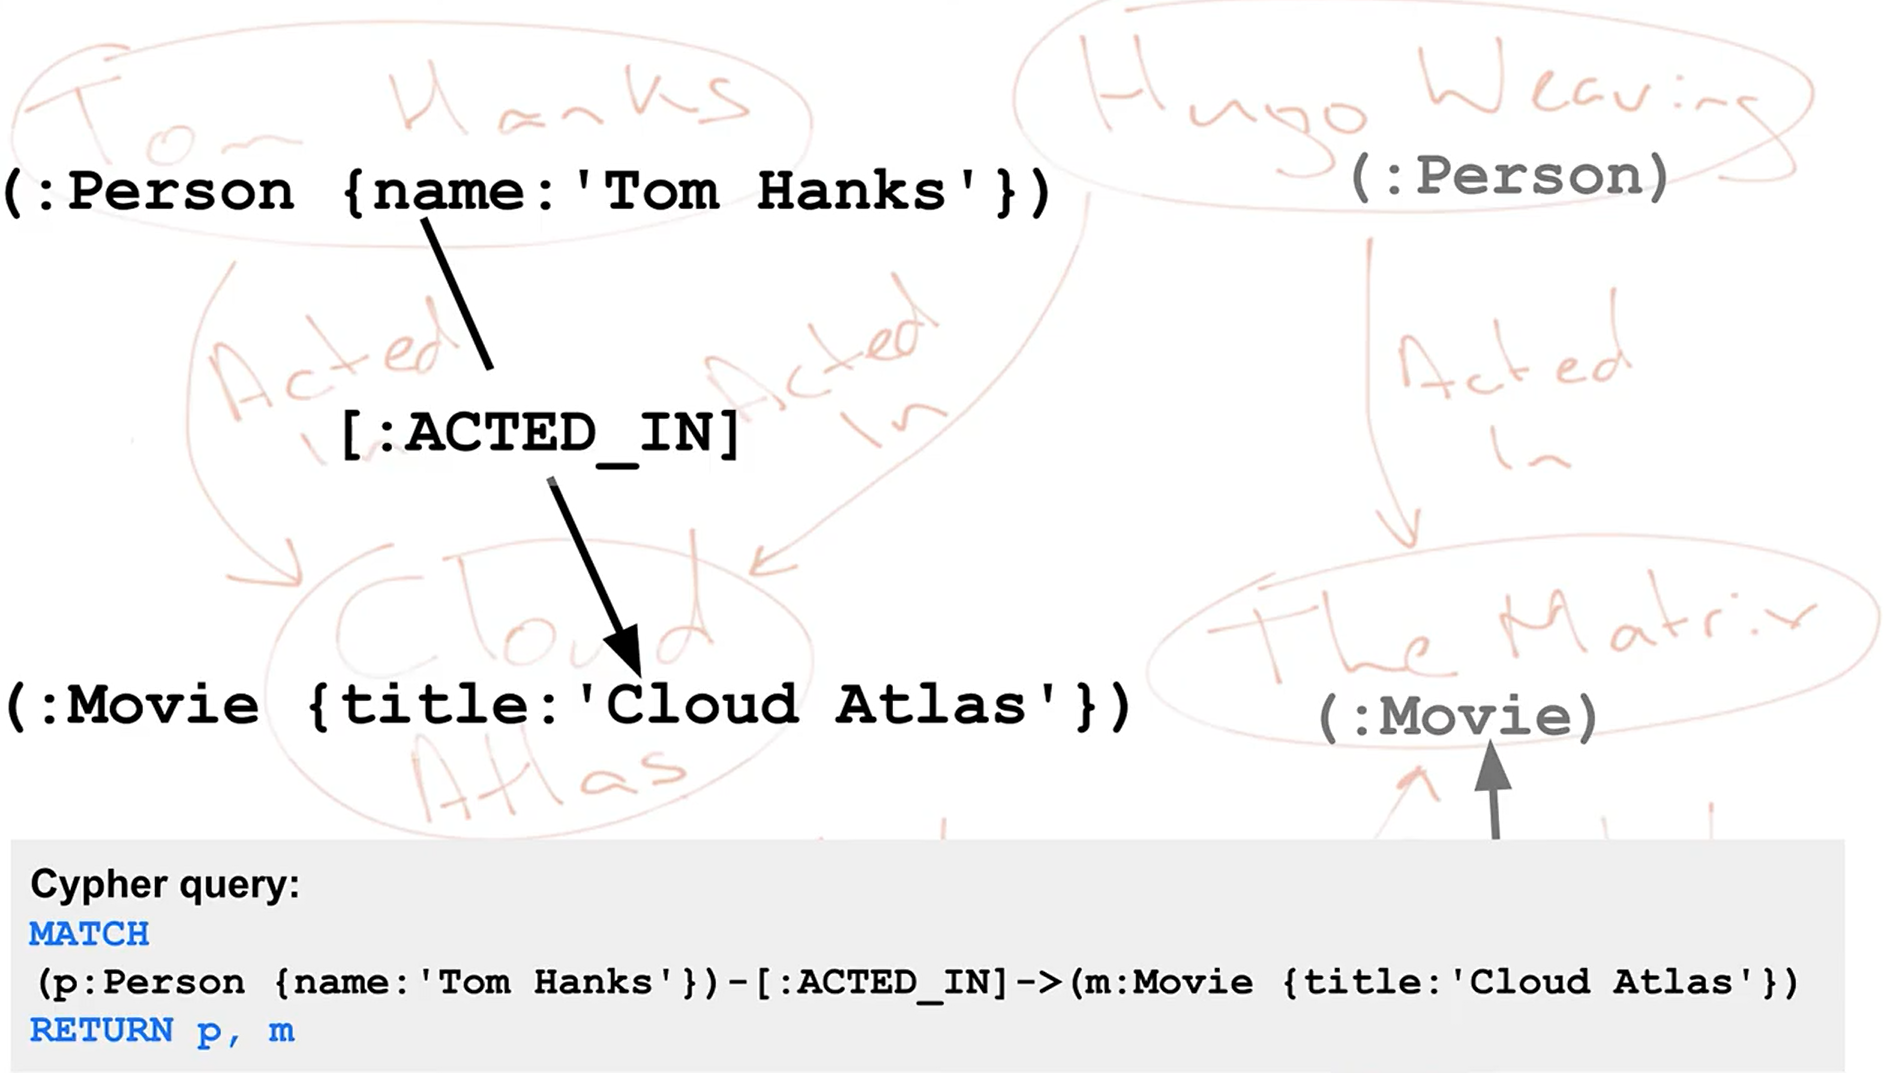
\includegraphics[width=0.8\linewidth,keepaspectratio]{neo4j64}
\end{center}	  


{\tiny (Ref: Introduction to cypher fundamentals  - neo4j)}

\end{frame}

%%%%%%%%%%%%%%%%%%%%%%%%%%%%%%%%%%%%%%%%%%%%%%%%%%%%%%%%%%%
\begin{frame}[fragile]\frametitle{Retrieval}

WHERE can be used to add logical expression, which is not possible in MATCH

\begin{center}
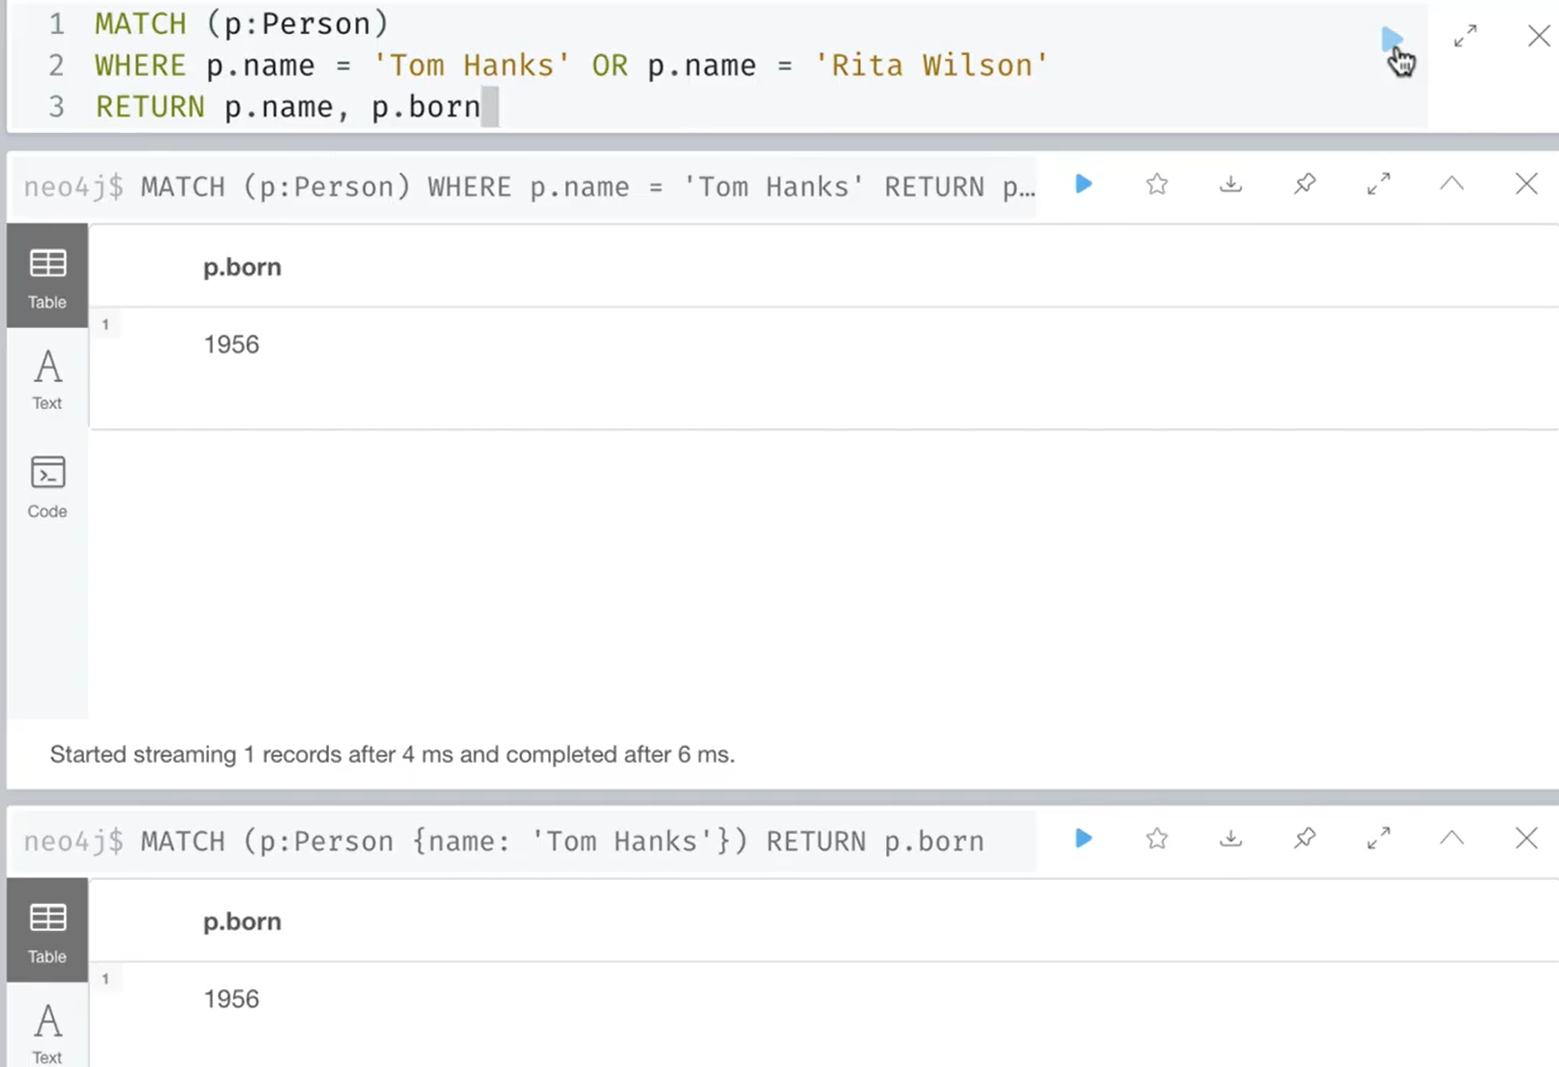
\includegraphics[width=0.8\linewidth,keepaspectratio]{neo4j65}
\end{center}	  


{\tiny (Ref: Introduction to cypher fundamentals  - neo4j)}

\end{frame}



%%%%%%%%%%%%%%%%%%%%%%%%%%%%%%%%%%%%%%%%%%%%%%%%%%%%%%%%%%%
\begin{frame}[fragile]\frametitle{MATCH}

Retrieve nodes

\begin{center}
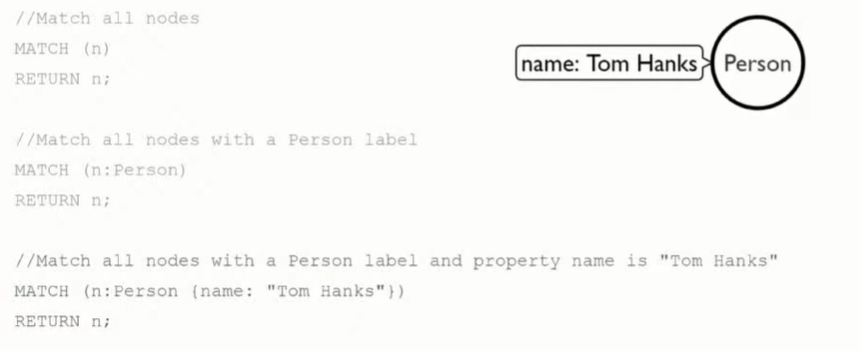
\includegraphics[width=\linewidth,keepaspectratio]{neo4j10}
\end{center}	  


{\tiny (Ref: Introduction to Neo4j - a hands-on crash course  - neo4j)}

\end{frame}

%%%%%%%%%%%%%%%%%%%%%%%%%%%%%%%%%%%%%%%%%%%%%%%%%%%%%%%%%%%
\begin{frame}[fragile]\frametitle{MATCH}

Retrieve nodes with properties

\begin{center}
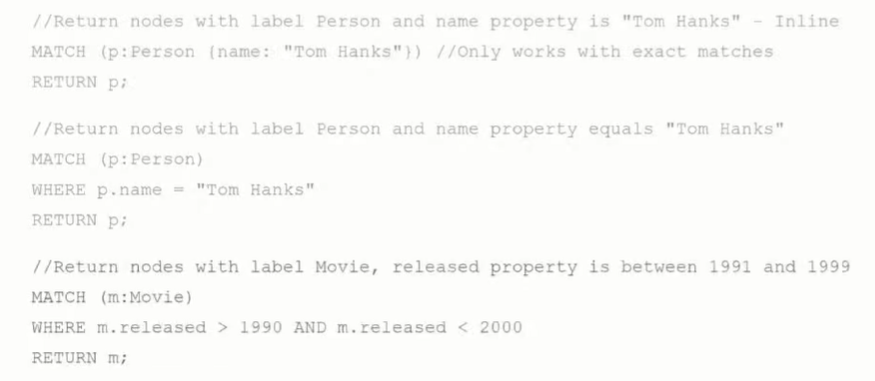
\includegraphics[width=\linewidth,keepaspectratio]{neo4j11}
\end{center}	  


{\tiny (Ref: Introduction to Neo4j - a hands-on crash course  - neo4j)}

\end{frame}

%%%%%%%%%%%%%%%%%%%%%%%%%%%%%%%%%%%%%%%%%%%%%%%%%%%%%%%%%%%
\begin{frame}[fragile]\frametitle{MATCH}

Retrieve nodes with relationships

\begin{center}
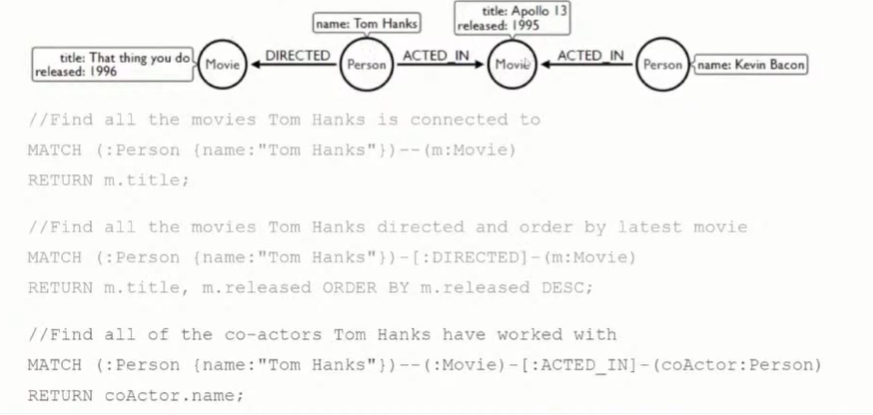
\includegraphics[width=\linewidth,keepaspectratio]{neo4j12}
\end{center}	  


{\tiny (Ref: Introduction to Neo4j - a hands-on crash course  - neo4j)}

\end{frame}

%%%%%%%%%%%%%%%%%%%%%%%%%%%%%%%%%%%%%%%%%%%%%%%%%%%%%%%%%%%
\begin{frame}[fragile]\frametitle{Retrieval}


\begin{itemize}
\item Absence of a property can also be checked in WHERE clause
\item Partial matches are allowed using STARTS\_WITH, ENDS\_WITH keywords
\item String tests are case sensitive, so better to LOWER them.
\item Check presence IN a list
\end{itemize}


\begin{center}
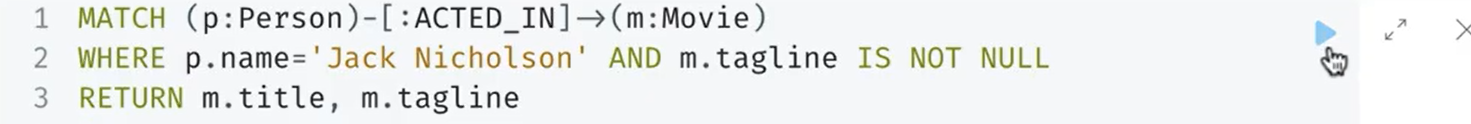
\includegraphics[width=\linewidth,keepaspectratio]{neo4j66}

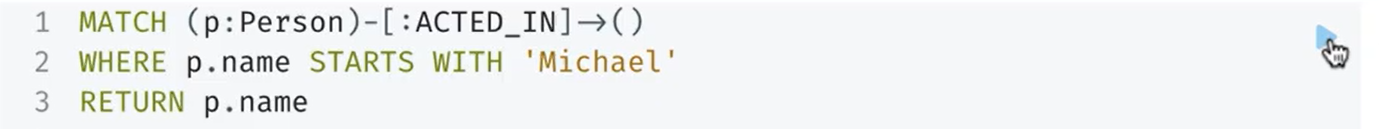
\includegraphics[width=\linewidth,keepaspectratio]{neo4j67}

\end{center}	  


{\tiny (Ref: Introduction to cypher fundamentals  - neo4j)}

\end{frame}

%%%%%%%%%%%%%%%%%%%%%%%%%%%%%%%%%%%%%%%%%%%%%%%%%%%%%%%%%%%
\begin{frame}[fragile]\frametitle{Aggregates}

\begin{itemize}
\item No need to specify grouping key. There is no group-by statement. Other Aggregates are SUM, STDDEV, etc.
\item Useful when you want to count the number of occurrences of a particular query result. It's possible to specify the occurrences of an alias count(n) and the graph engine calculates the number of occurrences of n. If we want to calculates the number of rows retrieved, including those with null values the count argument need to be a *. Last one is the count() without argument and this will implicit group by based upon the aggregation.
\end{itemize}

{\tiny (Ref: Learning Neo4j - Wabri Github)}


\begin{lstlisting}
// implicitly groups by p.name
MATCH (p.Person)-[:ACTED_IN]->(m:Movie)
RETURN p.name, count(*) AS numberOfMovies
\end{lstlisting}	

\end{frame}

%%%%%%%%%%%%%%%%%%%%%%%%%%%%%%%%%%%%%%%%%%%%%%%%%%%%%%%%%%%%%%%%%%%%%%%%%%%%%%%%%%
\begin{frame}\frametitle{Properties }

\begin{itemize}
\item Properties can be used to filter queries so that a subset of the graph is retrieved. \lstinline|CALL db.propertyKeys|
\item Nodes properties filtering \lstinline|MATCH (variable:Label {propertyKey1: propertyValue1, propertyKey2: propertyValue2}) RETURN variable|
\item In addition, with the RETURN clause, you can return property values from the retrieved nodes, rather than the nodes. \lstinline|MATCH (variable {property1: value}) RETURN variable.property2|
\end{itemize}


{\tiny (Ref: Learning Neo4j - Wabri Github)}
\end{frame}

%%%%%%%%%%%%%%%%%%%%%%%%%%%%%%%%%%%%%%%%%%%%%%%%%%%%%%%%%%%%%%%%%%%%%%%%%%%%%%%%%%
\begin{frame}\frametitle{Aliases }

\begin{itemize}
\item To customize the headings for a table containing property value it can be use aliases: \lstinline|MATCH (variable:Label {property1: value, property2: value}) RETURN variable.property2 AS alias1, variable.property3 AS alias2|
\item In the graph database we can specify aliases for the returned property values: \lstinline|MATCH (p:Person {born: 1970}) RETURN p.name AS name, p.born AS 'birth year'|
\end{itemize}


{\tiny (Ref: Learning Neo4j - Wabri Github)}
\end{frame}

%%%%%%%%%%%%%%%%%%%%%%%%%%%%%%%%%%%%%%%%%%%%%%%%%%%%%%%%%%%%%%%%%%%%%%%%%%%%%%%%%%
\begin{frame}\frametitle{Relationships}

The relationship can be specified with or without direction.

\begin{itemize}
\item \lstinline|() // a node|
\item \lstinline|()--() // 2 nodes have some type of relationship|
\item \lstinline|()-->() // the first node has a relationship to the second node|
\item \lstinline|()<--() // the second node has a relationship to the first node |
\end{itemize}

{\tiny (Ref: Learning Neo4j - Wabri Github)}
\end{frame}

%%%%%%%%%%%%%%%%%%%%%%%%%%%%%%%%%%%%%%%%%%%%%%%%%%%%%%%%%%%%%%%%%%%%%%%%%%%%%%%%%%
\begin{frame}\frametitle{Style recommendations}

\begin{itemize}
\item Node labels are CamelCase and begin with an upper-case letter, like Person or NetworkAddress.
\item Property keys, variables, parameters, aliases, and functions are camelCase and begin with a lower-case letter, like title or businessAddress.
\item Relationship type are in upper-case and can use the underscore, like ACTED\_IN or FOLLOWS.
\item Cypher keywords are upper-case, like MATCH or RETURN.
\item String constants are in single quotes, unless the string contains a quote or apostrophe, like 'The Matrix' or ``Somethings Gotta Give''.
\item Specify variables only when needed for use later in the cypher statement.
\item Place named nodes and relationships before anonymous nodes and relationships in the MATCH clauses when possible.
\item Specify anonymous relationships with \lstinline|-->, --, or <--|
\end{itemize}

{\tiny (Ref: Learning Neo4j - Wabri Github)}
\end{frame}

%%%%%%%%%%%%%%%%%%%%%%%%%%%%%%%%%%%%%%%%%%%%%%%%%%%%%%%%%%%%%%%%%%%%%%%%%%%%%%%%%%
\begin{frame}[fragile]\frametitle{Multiple Match patterns}

The MATCH clause includes a pattern specified by two paths separated by a comma:

\begin{lstlisting}
MATCH (a:Person)-[:ACTED_IN]->(m:Movie),
    (m:Movie)<-[:DIRECTED]-(d:Person)
WHERE m.released = 2000
RETURN a.name, m.title, d.name
\end{lstlisting}

\end{frame}

%%%%%%%%%%%%%%%%%%%%%%%%%%%%%%%%%%%%%%%%%%%%%%%%%%%%%%%%%%%%%%%%%%%%%%%%%%%%%%%%%%
\begin{frame}[fragile]\frametitle{Setting path variables}

It's possible to assign to a variable a path that can be reuse later in the same query or if it's needed to return that path:


\begin{lstlisting}
MATCH megPath = (meg:Person)-[:ACTED_IN]->(m:Movie)<-[:DIRECTED]-(d:Person),
    (other:Person)-[:ACTED_IN]->(m)
WHERE meg.name = 'Meg Ryan'
RETURN megPath
\end{lstlisting}

\end{frame}

%%%%%%%%%%%%%%%%%%%%%%%%%%%%%%%%%%%%%%%%%%%%%%%%%%%%%%%%%%%%%%%%%%%%%%%%%%%%%%%%%%
\begin{frame}[fragile]\frametitle{Varying length paths}

It's possible to assign to a variable a path that can be reuse later in the same query or if it's needed to return that path:


\begin{itemize}
\item Any graph that represents social networking, trees, or hierarchies will most likely have multiple paths of varying lengths.

\item To get this far you need to use this format \lstinline|(nodeA)-[:REALTYPE*<number_of_hops>]->(nodeB) or (nodeA)-[:REALTYPE*n..m]->(nodeB)| where n and m are the extremes of an interval.
\end{itemize}

{\tiny (Ref: Learning Neo4j - Wabri Github)}
\end{frame}

%%%%%%%%%%%%%%%%%%%%%%%%%%%%%%%%%%%%%%%%%%%%%%%%%%%%%%%%%%%%%%%%%%%%%%%%%%%%%%%%%%
\begin{frame}[fragile]\frametitle{Finding the shortest path}

A built-in function that you may find useful in a graph that has many ways of traversing the graph to get to the same node is the shortestPath() function. Using the shortest path between two nodes improves the performance of the query.

\begin{lstlisting}
MATCH p = shortestPath((m1:Movie)-[*]-(m2:Movie))
WHERE m1.title = 'A Few Good Men' AND
    m2.title = 'The Matrix'
RETURN p
\end{lstlisting}

\end{frame}

%%%%%%%%%%%%%%%%%%%%%%%%%%%%%%%%%%%%%%%%%%%%%%%%%%%%%%%%%%%%%%%%%%%%%%%%%%%%%%%%%%
\begin{frame}[fragile]\frametitle{Optional pattern matching}
This clause OPTIONAL MATCH is just like the MATCH but if no matches are found, this clause will use null for missing parts of the pattern. Here is an examples:

\begin{lstlisting}
MATCH (p:Person)
WHERE p.name STARTS WITH 'James'
OPTIONAL MATCH (p)-[r:REVIEWED]->(m:Movie)
RETURN p.name, type(r), m.title
\end{lstlisting}


\begin{center}
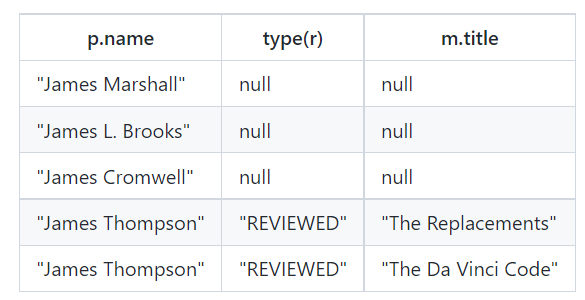
\includegraphics[width=0.4\linewidth,keepaspectratio]{neo4j83}
\end{center}	


{\tiny (Ref: Learning Neo4j - Wabri Github)}
\end{frame}

%%%%%%%%%%%%%%%%%%%%%%%%%%%%%%%%%%%%%%%%%%%%%%%%%%%%%%%%%%%%%%%%%%%%%%%%%%%%%%%%%%
\begin{frame}[fragile]\frametitle{Collecting results }

Cypher has a built-in function collect() that enables you to aggregate value into a list and the result will be a list called movies for Tom Cruise with the values ["Jerry Maguire", "Top Gun", "A Few Good Men"].

\begin{lstlisting}
MATCH (p:Person)-[:ACTED_IN]->(m:Movie)
WHERE p.name = 'Tom Cruise'
RETURN collect(m.title) AS `movies for Tom Cruise`
\end{lstlisting}


\end{frame}

%%%%%%%%%%%%%%%%%%%%%%%%%%%%%%%%%%%%%%%%%%%%%%%%%%%%%%%%%%%%%%%%%%%%%%%%%%%%%%%%%%
\begin{frame}[fragile]\frametitle{Additional processing using WITH}

\begin{itemize}
\item During the execution of a MATCH clause, is possible to specify some intermediate calculations or values that will be used for further processing of the query, or for limiting the number of results before further processing is done. With the WITH clause it's possible to perform intermediate processing of data flow operations.
\item This example return the actors name only if they acted on 2 or 3 movies, with a reference of the numbers of the films and a list of that.
\item Be careful with this clause because in the WITH body are specify some variables from the previous part of the query that need to be part of the next section of the query, all the aliases for the next part are the only one defined in the body.
\end{itemize}

\begin{lstlisting}
MATCH (a:Person)-[:ACTED_IN]->(m:Movie)
WITH a, count(a) AS numMovies, collect(m.title) AS movies
WHERE numMovies > 1 AND numMovies < 4
RETURN a.name, numMovies, movies
\end{lstlisting}

\end{frame}

%%%%%%%%%%%%%%%%%%%%%%%%%%%%%%%%%%%%%%%%%%%%%%%%%%%%%%%%%%%%%%%%%%%%%%%%%%%%%%%%%%
\begin{frame}[fragile]\frametitle{Additional processing using WITH}

Remember to name all expressions with an alias in a WITH that are not simple variables. This is a simple query to retrieve all the actor that are acted in at least 5 movies and if they also directed a movie than return the name of that movie.


\begin{lstlisting}
MATCH (p:Person)
WITH p, size((p)-[:ACTED_IN]->(:Movie)) as movies
WHERE movies>=5
OPTIONAL MATCH (p)-[:DIRECTED]->(m:Movie)
RETURN p.name, m.title

\end{lstlisting}


\begin{center}
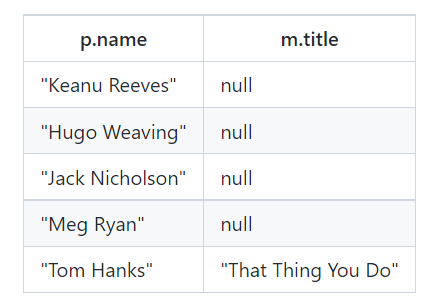
\includegraphics[width=0.4\linewidth,keepaspectratio]{neo4j84}
\end{center}	


{\tiny (Ref: Learning Neo4j - Wabri Github)}
\end{frame}

%%%%%%%%%%%%%%%%%%%%%%%%%%%%%%%%%%%%%%%%%%%%%%%%%%%%%%%%%%%%%%%%%%%%%%%%%%%%%%%%%%
\begin{frame}[fragile]\frametitle{Eliminating duplication}

To eliminating duplicated results it can be used the DISTINCT keyword



\begin{lstlisting}
MATCH (gene:Person)-[:ACTED_IN]->(movie:Movie)
WHERE gene.name = 'Gene Hackman'
OPTIONAL MATCH
    (other:Person)-[:ACTED_IN]->(movie),
    (dir:Person)-[:DIRECTED]->(movie)
WITH
    movie,
    collect(other.name) AS Actors,
    collect(DISTINCT dir.name) AS Directors
RETURN
    movie.title AS `Title of movie`,
    Actors AS `Co-Actors`,
    Directors

\\ can be use in several uses, like this:

MATCH (p:Person)-[:DIRECTED | :ACTED_IN]->(m:Movie)
WHERE p.name = 'Tom Hanks'
WITH DISTINCT m
RETURN m.released, m.title
\end{lstlisting}

\end{frame}

%%%%%%%%%%%%%%%%%%%%%%%%%%%%%%%%%%%%%%%%%%%%%%%%%%%%%%%%%%%%%%%%%%%%%%%%%%%%%%%%%%
\begin{frame}[fragile]\frametitle{Ordering result}

If you want the results to be sorted, you specify the expression to use for the sort usign the ORDER BY keyword and whether you want the order to be descending using the DESC keyword.


\begin{lstlisting}
MATCH (p:Person)-[:DIRECTED | :ACTED_IN]->(m:Movie)
WHERE p.name = 'Tom Hanks' AND m.released >= 2000
RETURN m.released, collect(DISTINCT m.title) AS movies ORDER BY m.released DESC
//
\end{lstlisting}

\begin{center}
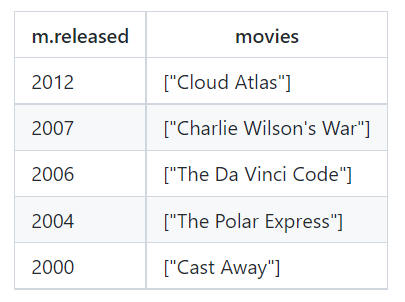
\includegraphics[width=0.4\linewidth,keepaspectratio]{neo4j85}
\end{center}	  


{\tiny (Ref: Learning Neo4j - Wabri Github)}
\end{frame}

%%%%%%%%%%%%%%%%%%%%%%%%%%%%%%%%%%%%%%%%%%%%%%%%%%%%%%%%%%%%%%%%%%%%%%%%%%%%%%%%%%
\begin{frame}[fragile]\frametitle{Limiting the number of results}

Although you can filter queries to reduce the number of results returned, you may also want to limit the number of results. This is useful if you have very large result sets and you only need to see the beginning or end of a set of ordered results. LIMIT is the right choice to do something like this.

\begin{lstlisting}
MATCH (m:Movie)
RETURN m.title as title, m.released as year
ORDER BY m.released DESC
LIMIT 10
\end{lstlisting}


\end{frame}


%%%%%%%%%%%%%%%%%%%%%%%%%%%%%%%%%%%%%%%%%%%%%%%%%%%%%%%%%%%%%%%%%%%%%%%%%%%%%%%%%%
\begin{frame}[fragile]\frametitle{List}

A Cypher map is list of key/value pairs where each element of the list is of the format key: value.

It's possible to collect values for a list during a query and with this it's possible to sort by the size of the list using the size() function as follows:

\begin{lstlisting}
MATCH (a:Person)-[:ACTED_IN]->(m:Movie)
WITH m, count(m) AS numCast, collect(a.name) AS cast
RETURN m.title, cast, numCast
ORDER BY size(cast)
\end{lstlisting}


\end{frame}



%%%%%%%%%%%%%%%%%%%%%%%%%%%%%%%%%%%%%%%%%%%%%%%%%%%%%%%%%%%%%%%%%%%%%%%%%%%%%%%%%%
\begin{frame}[fragile]\frametitle{Unwinding lists}

There my be some situations where you want to perform the opposite of collecting results, but rather separate the lists into separate rows. This functionality is done using the unwind clause.

Here is an example where we create a list with three elements, unwind the list and then return the values. Since there are three elements, three rows are returned with the values:

\begin{lstlisting}
WITH [1, 2, 3] AS list
UNWIND list AS row
RETURN row, list
//
\end{lstlisting}


\begin{center}
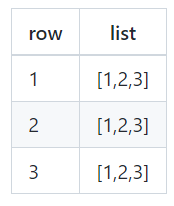
\includegraphics[width=0.2\linewidth,keepaspectratio]{neo4j86}
\end{center}	 

The unwind clause is frequently used when importing data into a graph.

 

{\tiny (Ref: Learning Neo4j - Wabri Github)}
\end{frame}

%%%%%%%%%%%%%%%%%%%%%%%%%%%%%%%%%%%%%%%%%%%%%%%%%%%%%%%%%%%%%%%%%%%%%%%%%%%%%%%%%%
\begin{frame}[fragile]\frametitle{Dates}

Cypher has a built-in date() function, as well as other temporal values and functions that you can use to calculate temporal values. You use a combination of numeric, temporal, spatial, list and string functions to calculate values that are useful to your application.

For example we want to calculate all the age value of the actors given the born year:

\begin{lstlisting}
MATCH (actor:Person)-[:ACTED_IN]->(:Movie)
WHERE exists(actor.born)
WITH DISTINCT actor, date().year - actor.born AS age
RETURN actor.name, age AS `age today`
ORDER BY actor.born DESC
\end{lstlisting}

\end{frame}



%%%%%%%%%%%%%%%%%%%%%%%%%%%%%%%%%%%%%%%%%%%%%%%%%%%%%%%%%%%
\begin{frame}[fragile]\frametitle{Complex Example}
A Social Recommendation

\begin{center}
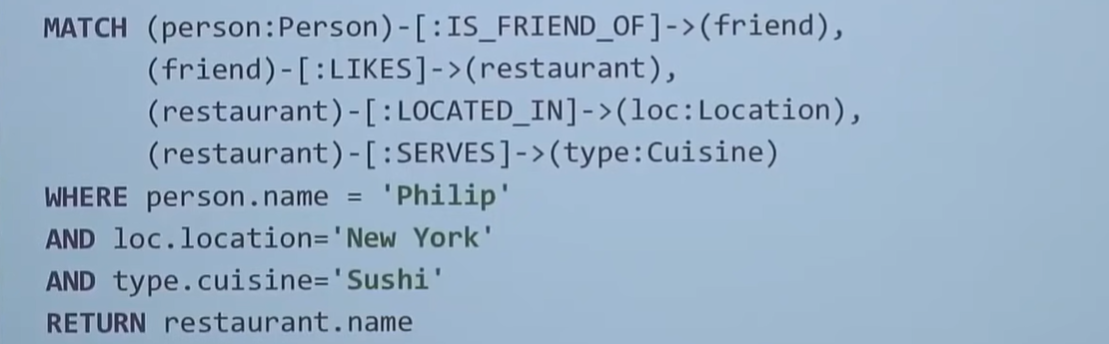
\includegraphics[width=\linewidth,keepaspectratio]{neo4j15}
\end{center}	  


{\tiny (Ref: Introduction to Neo4j and Graph Databases
 - M David Allen)}

\end{frame}



%%%%%%%%%%%%%%%%%%%%%%%%%%%%%%%%%%%%%%%%%%%%%%%%%%%%%%%%%%%
\begin{frame}[fragile]\frametitle{Complex Example}
What are the top 10 jobs for me, that are same location as I am in and also for which I have necessary qualifications?

\begin{center}
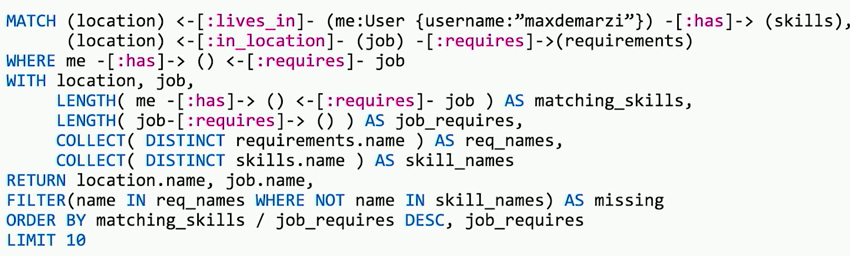
\includegraphics[width=\linewidth,keepaspectratio]{neo4j27}
\end{center}	    



{\tiny (Ref: Secret Sauce of Neo4j: Modeling and Querying Graphs
 - Max De Marzi )}

\end{frame}

%%%%%%%%%%%%%%%%%%%%%%%%%%%%%%%%%%%%%%%%%%%%%%%%%%%%%%%%%%%
\begin{frame}[fragile]\frametitle{Answer}

Partial sub-graph match

\begin{center}
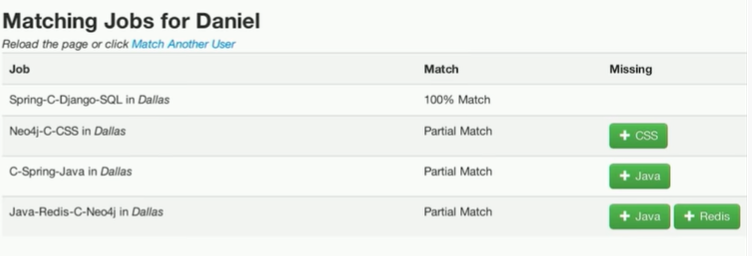
\includegraphics[width=\linewidth,keepaspectratio]{neo4j28}
\end{center}	    


{\tiny (Ref: Secret Sauce of Neo4j: Modeling and Querying Graphs
 - Max De Marzi )}

\end{frame}

%%%%%%%%%%%%%%%%%%%%%%%%%%%%%%%%%%%%%%%%%%%%%%%%%%%%%%%%%%%%%%%%%%%%%%%%%%%%%%%%%%
\begin{frame}[fragile]\frametitle{}
\begin{center}
{\Large Writing}
\end{center}
\end{frame}



%%%%%%%%%%%%%%%%%%%%%%%%%%%%%%%%%%%%%%%%%%%%%%%%%%%%%%%%%%%
\begin{frame}[fragile]\frametitle{Nodes}

\begin{itemize}
\item MERGE: Creates a new node if not present already. All subsequent calls do not do anything as node with said properties is already present.

\item CREATE: Will create multiple nodes even if nodes with similar properties are present already
\end{itemize}

\begin{center}
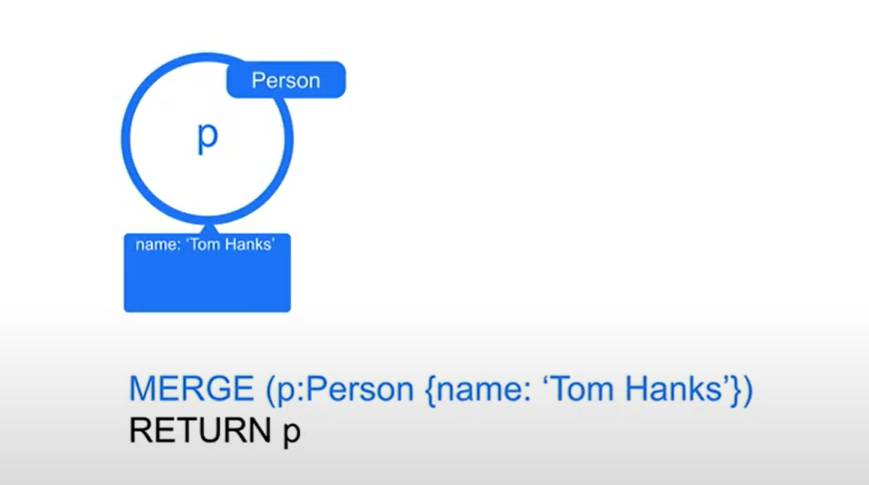
\includegraphics[width=0.5\linewidth,keepaspectratio]{neo4j68}
\end{center}	  


{\tiny (Ref: Introduction to cypher fundamentals  - neo4j)}

\end{frame}

%%%%%%%%%%%%%%%%%%%%%%%%%%%%%%%%%%%%%%%%%%%%%%%%%%%%%%%%%%%
\begin{frame}[fragile]\frametitle{Nodes}


\begin{center}
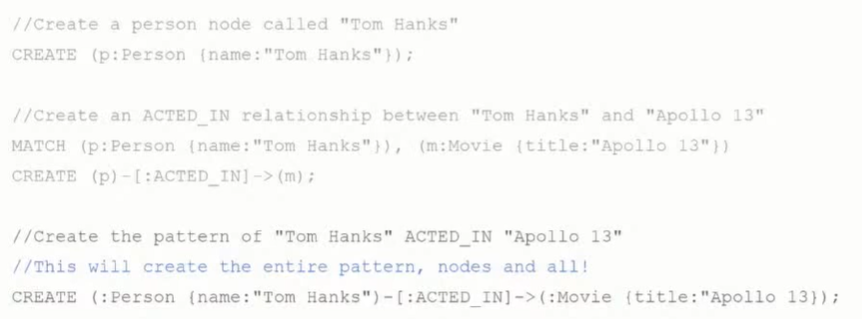
\includegraphics[width=\linewidth,keepaspectratio]{neo4j13}
\end{center}	  


{\tiny (Ref: Introduction to Neo4j - a hands-on crash course  - neo4j)}

\end{frame}


%%%%%%%%%%%%%%%%%%%%%%%%%%%%%%%%%%%%%%%%%%%%%%%%%%%%%%%%%%%
\begin{frame}[fragile]\frametitle{Relationships}

\begin{itemize}
\item First get two existing nodes between which a relationship needs to be created.
\item Same MERGE logic is there for Relationships as well.
item Relationship type must begin with ':'
\end{itemize}

\begin{center}
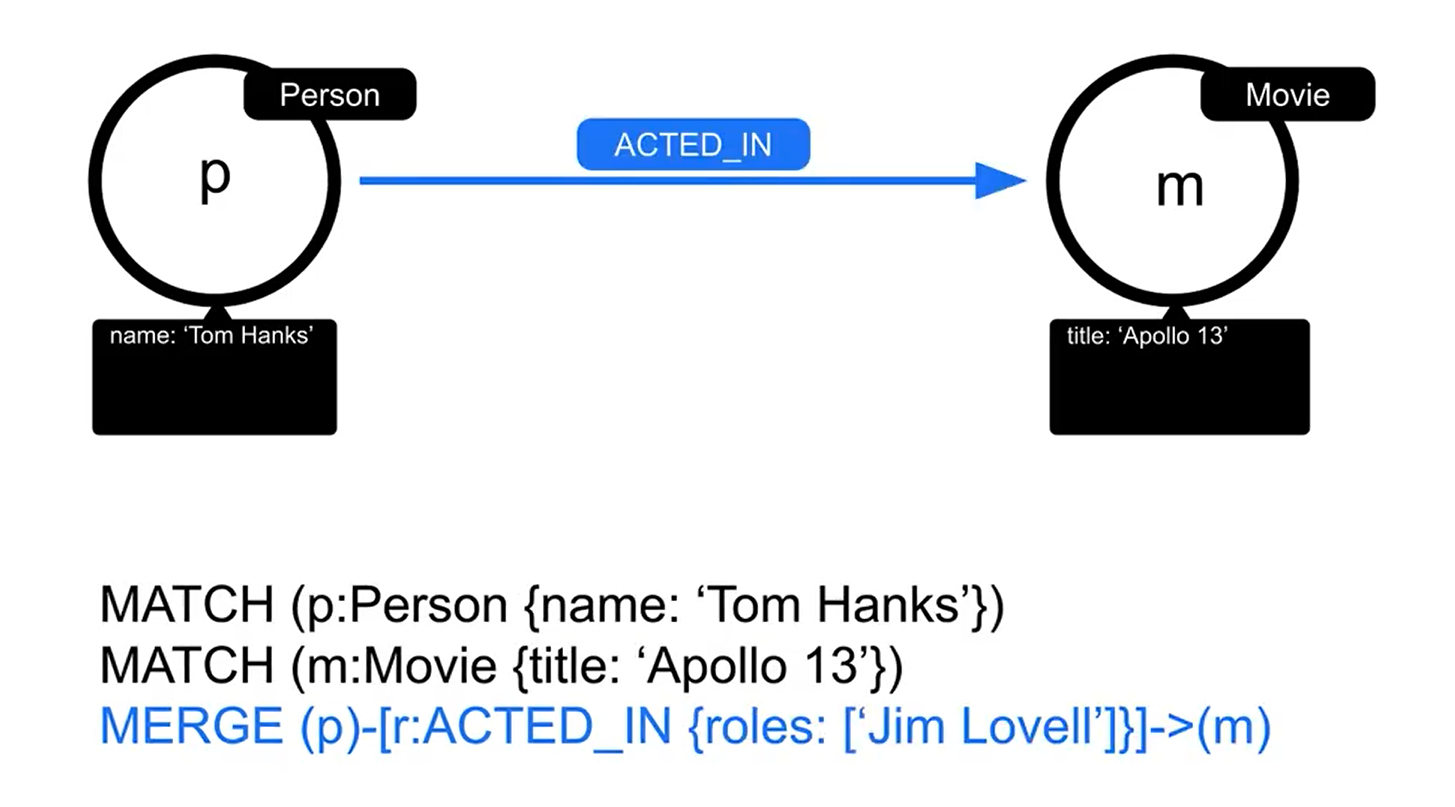
\includegraphics[width=0.8\linewidth,keepaspectratio]{neo4j69}
\end{center}	  


{\tiny (Ref: Introduction to cypher fundamentals  - neo4j)}

\end{frame}

%%%%%%%%%%%%%%%%%%%%%%%%%%%%%%%%%%%%%%%%%%%%%%%%%%%%%%%%%%%
\begin{frame}[fragile]\frametitle{Properties}

\begin{itemize}
\item Use SET to set new or existing properties
\item It can be used for both Nodes and Relationships
\item Use REMOVE to remove a property. (it should not be a primary key though)
\end{itemize}

\begin{center}
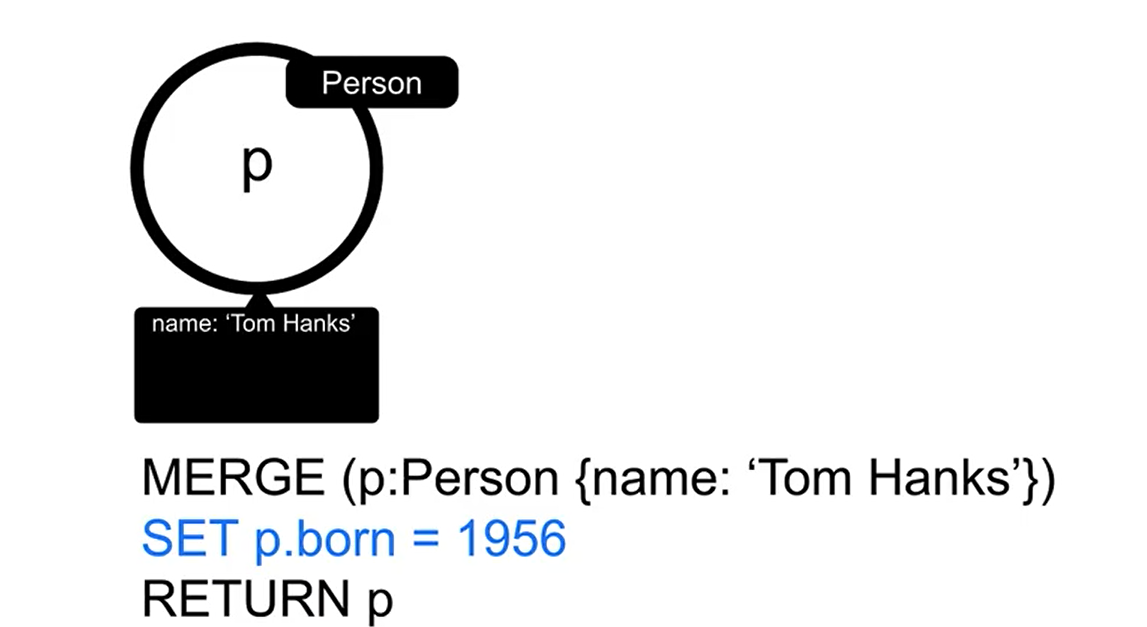
\includegraphics[width=0.5\linewidth,keepaspectratio]{neo4j70}
\end{center}	  


{\tiny (Ref: Introduction to cypher fundamentals  - neo4j)}

\end{frame}


%%%%%%%%%%%%%%%%%%%%%%%%%%%%%%%%%%%%%%%%%%%%%%%%%%%%%%%%%%%
\begin{frame}[fragile]\frametitle{Constrains}
We add a uniqueness constraint to the graph by creating a constraint that asserts that a particular node property is unique in the graph for a particular type of node.

\begin{lstlisting}
// to ensure uniqueness and fast lookups
CREATE CONSTRAINT ON (label:Label)
ASSERT label.property IS UNIQUE

// This statement will fail if the graph already has multiple Movie nodes with the same value for the title property.

// We can also create a constraint on properties of relationships, its not necessary to define the direction of the relationship:

CREATE CONSTRAINT ON ()-[rel:REVIEWED]-() ASSERT exists(rel.rating)
\end{lstlisting}	  


\end{frame}

%%%%%%%%%%%%%%%%%%%%%%%%%%%%%%%%%%%%%%%%%%%%%%%%%%%%%%%%%%%
\begin{frame}[fragile]\frametitle{Conditionals}

\begin{itemize}
\item ON CREATE will do the SET at the time of creation, ie first time when the node is created. There ON MATCH wont run.
\item Next time, when the whole code is executed again, ON CRETAE wont run, but ON MATCH will.
\end{itemize}

\begin{center}
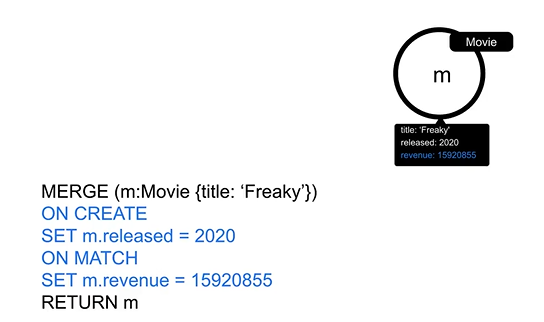
\includegraphics[width=0.8\linewidth,keepaspectratio]{neo4j71}
\end{center}	  


{\tiny (Ref: Introduction to cypher fundamentals  - neo4j)}
 

\end{frame}

%%%%%%%%%%%%%%%%%%%%%%%%%%%%%%%%%%%%%%%%%%%%%%%%%%%%%%%%%%%
\begin{frame}[fragile]\frametitle{Delete}

\begin{itemize}
\item Just get the reference to the object and delete it.
\item It can be a Node (if dangling) or a Relationship.
\item DETACH DELETE removes all relationships from the node and then DELETEs it.
\item To delete all nodes, just say \lstinline|MATCH (n) DETACH DELETE n|
\end{itemize}

\begin{center}
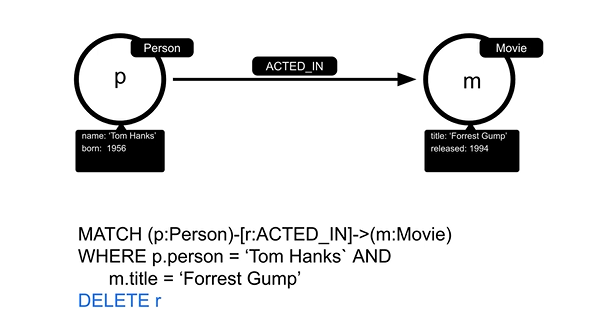
\includegraphics[width=0.8\linewidth,keepaspectratio]{neo4j72}
\end{center}	  


{\tiny (Ref: Introduction to cypher fundamentals  - neo4j)}
 

\end{frame}


%%%%%%%%%%%%%%%%%%%%%%%%%%%%%%%%%%%%%%%%%%%%%%%%%%%%%%%%%%%%%%%%%%%%%%%%%%%%%%%%%%
\begin{frame}[fragile]\frametitle{Parameters}

\begin{itemize}
\item In the Cypher statements, a parameter name begins with the \$ symbol.
\item At runtime, if the parameter \$actorName has a value, it will be used in the Cypher statement when it runs in the graph engine.
\item In Neo4j Browser to set values of parameters we can use the command :param:
\item \lstinline|:param actorName => 'Tom Hanks'|
\end{itemize}

\begin{lstlisting}
MATCH (p:Person)-[:ACTED_IN]->(m:Movie)
WHERE p.name = $actorName
RETURN m.released, m.title
ORDER BY m.released DESC
\end{lstlisting}

\end{frame}

%%%%%%%%%%%%%%%%%%%%%%%%%%%%%%%%%%%%%%%%%%%%%%%%%%%%%%%%%%%%%%%%%%%%%%%%%%%%%%%%%%
\begin{frame}[fragile]\frametitle{Explain Profile}

There are two Cypher keywords to use as prefix with a Cypher statement to analyze a query:
\begin{itemize}
\item EXPLAIN provides estimates of the graph engine processing that will occur, but does not execute the statement.
\item PROFILE provides real profiling information for what has occurred in the graph engine during the query and executes the statement.
\item This query return the phases of the Cypher execution, it can be possible to examine what code is expected to run. Each phase of the query presents an estimante of the number of rows expected to be returned.
\end{itemize}

\begin{lstlisting}
EXPLAIN
MATCH (p:Person)-[:ACTED_IN]->(m:Movie)
WHERE p.name = $actorName AND
      m.released < $year
RETURN p.name, m.title, m.released

\end{lstlisting}

\end{frame}


%%%%%%%%%%%%%%%%%%%%%%%%%%%%%%%%%%%%%%%%%%%%%%%%%%%%%%%%%%%%%%%%%%%%%%%%%%%%%%%%%%
\begin{frame}[fragile]\frametitle{Profile}

\begin{itemize}
\item For a better metric for analyzing how the Cypher statement will run is needed to run the PROFILE prefix keyword which runs the statement and gives the run-time performance metrics.
\item This query above show the cache hits and most importantly the number of times that the engine accessed the database (db hints). This is the metric that will affect the performance of the Cypher statement at run-time.
\end{itemize}

\begin{lstlisting}
PROFILE
MATCH (p:Person)-[:ACTED_IN]->(m:Movie)
WHERE p.name = $actorName AND
      m.released < $year
RETURN p.name, m.title, m.released
\end{lstlisting}



\end{frame}


%%%%%%%%%%%%%%%%%%%%%%%%%%%%%%%%%%%%%%%%%%%%%%%%%%%%%%%%%%%
\begin{frame}[fragile]\frametitle{Managing indexes}
The uniqueness and node key constraints are essentially single-property and composite indexes respectively. Indexes are used to improve initial node lookup performance, but they require additional storage in the graph to maintain and also add to the cost of creating or modifying property values that are indexed. Indexes store redundant data that points to nodes with the specific property value or values. Unlike SQL, there is no such thing as a primary key in Neo4j, but nodes can have multiple properties that must be unique. This are single-property indexes used:



\begin{itemize}
\item Equality checks: $=$
\item Range comparisons: $>,>=,<, <=$
\item List membership: IN
\item String comparisons: STARTS WITH, ENDS WITH, CONTAINS
\item Existence checks: exists()
\item Spatial distance searches: distance()
\item Spatial bounding searches: point()
\end{itemize}

Composite indexes are used only for equality checks and list membership.



{\tiny (Ref: Learning Neo4j - Wabri Github)}

\end{frame}

%%%%%%%%%%%%%%%%%%%%%%%%%%%%%%%%%%%%%%%%%%%%%%%%%%%%%%%%%%%
\begin{frame}[fragile]\frametitle{Managing indexes}
\begin{itemize}
\item The index for a property of a node can greatly reduce the number of nodes that the engine needs to visit in oredr to satisy a query.
\item The graph engine will find the pointers to all nodes that satisfy the query without having to visit all of the nodes:
\end{itemize}


\begin{lstlisting}
MATCH (m:Movie)
WHERE 1990 < m.released < 2000
SET m.videoFormat = 'DVD'
\end{lstlisting}

\end{frame}

%%%%%%%%%%%%%%%%%%%%%%%%%%%%%%%%%%%%%%%%%%%%%%%%%%%%%%%%%%%
\begin{frame}[fragile]\frametitle{From relational to graph}
To convert a relational database into a graph database with one step you can use the ETL tool (Extract Transform Load) $->$ Neo4J ETL

In Cypher it's possible to:

\begin{itemize}
\item Load data from a URL (http(s) or file)
\item Process data as a stream of records
\item Create or update the graph with the data being loaded
\item Use transactions during the data load
\item Transform and convert values from the load stream
\item Load up to 10M nodes and relationships
\end{itemize}

Commonly to import data into a graph is used the csv files, to do that it's necessary to develop a model that describes how data need to be represents in the graph.

{\tiny (Ref: Learning Neo4j - Wabri Github)}

\end{frame}

%%%%%%%%%%%%%%%%%%%%%%%%%%%%%%%%%%%%%%%%%%%%%%%%%%%%%%%%%%%
\begin{frame}[fragile]\frametitle{Importing normalized data}

The LOAD CSV clause parses a local in the import directory of the neo4j installation or a remote file into a stream of rows which represent maps (with eaders) or lists. Once done this it's possible to use Cypher operations to create nodes or relationships or merge existing graph.

\begin{itemize}
\item The row is a variable that is used to extract data from file.
\item The first line of the file must contain a comma-separated list of column names.
\item The url-value can be a resource or a file on the system.
\item Each line of this file must contains data that is interpreted as values for each column name. When each line is read from the file, it's possible to perform the necessary processing to create or merge data into the graph.
\end{itemize}

\begin{lstlisting}
LOAD CSV WITH HEADERS FROM url-value
AS row
\end{lstlisting}

\end{frame}

%%%%%%%%%%%%%%%%%%%%%%%%%%%%%%%%%%%%%%%%%%%%%%%%%%%%%%%%%%%
\begin{frame}[fragile]\frametitle{Importing normalized data}
Before loading data from CSV files into graph, we need to confirm that the data retrived looks ok. To do this we can first print the lines of the file and get some information about the data to be loaded.

\begin{lstlisting}
LOAD CSV WITH HEADERS
FROM 'http://data.neo4j.com/intro-neo4j/movies_to_load.csv'
as LINE
RETURN count(*)
\end{lstlisting}


\end{frame}


%%%%%%%%%%%%%%%%%%%%%%%%%%%%%%%%%%%%%%%%%%%%%%%%%%%%%%%%%%%
\begin{frame}[fragile]\frametitle{Importing de-normalized data}
When file that we need to import are de-normalized a supplementary step is needed.


There are a specifications for the field terminator of the file, this is an example:

\begin{lstlisting}
title;released;summary;actor;birthyear;characters
Back to the Future;1985;17 year old Marty McFly got home early last night. 30 years early.;Michael J. Fox;1961;Marty McFly
Back to the Future;1985;17 year old Marty McFly got home early last night. 30 years early.;Christopher Lloyd;1938;Dr. Emmet Brown

// From this we want to create person and movies:

LOAD CSV WITH HEADERS
FROM 'https://data.neo4j.com/intro-neo4j/movie_actor_roles_to_load.csv'
AS line FIELDTERMINATOR ';'
MERGE (movie:Movie { title: line.title })
ON CREATE SET movie.released = toInteger(line.released),
              movie.tagline = line.summary
MERGE (actor:Person { name: line.actor })
ON CREATE SET actor.born = toInteger(line.birthyear)
MERGE (actor)-[r:ACTED_IN]->(movie)
ON CREATE SET r.roles = split(line.characters,',')
\end{lstlisting}


\end{frame}

%%%%%%%%%%%%%%%%%%%%%%%%%%%%%%%%%%%%%%%%%%%%%%%%%%%%%%%%%%%
\begin{frame}[fragile]\frametitle{Importing de-normalized data}

Two main things to notice:

\begin{itemize}
\item the definition of the semi-colon as a field terminator rather than comma;
\item the build-in method split() to create the list for the roles property.
\end{itemize}

To import a larger amount of data (more than 10k rows), it is recommended to prefix the load csv clause with a PERIODIC COMMIT hint. This allow the database to regularly commit the import transactions to avoid memory churn for large transaction-states.

{\tiny (Ref: Learning Neo4j - Wabri Github)}

\end{frame}
